\documentclass[a4paper,onecolumn,12pt]{jsarticle}

\usepackage{hamacro}
\hypersetup{
  pdfstartview={FitH},
  pdftitle={タイトル},
  pdfauthor={著者},
  pdfsubject={サブタイトル},
  pdfkeywords={キーワード},
}

% title
\title{\LaTeX テンプレート}
\author{HAMANO Tsukasa}
\date{\today}

% document
\begin{document}
\maketitle
\vspace{1em}
\tableofcontents
\clearpage

\section{修飾}

formatting by \emph{emph}

formatting by \textbf{textbf}

emphによる\emph{強調}

textbfによる\textbf{強調}

\subsection{フォントサイズ}

\tiny{あ tiny}\\
\scriptsize{あ scriptsize}\\
\footnotesize{あ footnotesize}\\
\small{あ small}\\
\normalsize{あ normalsize}\\
\large{あ large}\\
\Large{あ Large}\\
\LARGE{あ LARGE}\\
\huge{あ huge}\\
\Huge{あ Huge}\\
\normalsize{リセット}\\

\subsection{リンク}
\url{http://localhost/}

\href{http://www.example.com/}{example.com}

\section{リスト}

\subsection{itemaize}
\begin{itemize}
\item その1
\item その2
\item その3
\end{itemize}

\subsection{enumerate}
\begin{enumerate}
\item その1
\item その2
\item その3
\end{enumerate}

\subsection{description}
\begin{description}
  \item[名前1] 説明1
  \item[名前2] 説明2
  \item[名前3] 説明3
\end{description}

\section{引用}

\subsection{quote}
字下げなし
\begin{quote}
1行目

2行目

3行目
\end{quote}

\subsection{quotation}
字下げあり
\begin{quotation}
1行目

2行目

3行目
\end{quotation}

\section{ソースコード}


hello.c

\begin{verbatim}
#include <stdio.h>

int main(int argc, char *argv[]){
    printf("Hello World!\n");
    return 0;
}
\end{verbatim}

\section{テーブル}
\subsection{普通のテーブル}
\begin{tabular}{|l|c|r|}
\hline
セル1 & セル2 & セル3 \\ \hline
セル4 & セル5 & セル6 \\ \hline
セル7 & セル8 & セル9 \\ \hline
\end{tabular}

\subsection{タイトル付きテーブル(中央)}

\begin{table}[htbp]
\begin{center}
\begin{tabular}{|l|c|r|}
\hline
セル1 & セル2 & セル3 \\ \hline
セル4 & セル5 & セル6 \\ \hline
セル7 & セル8 & セル9 \\ \hline
\end{tabular}
\caption{タイトル}
\end{center}
\end{table}

\subsection{水平線}
\begin{center}\rule{3in}{0.4pt}\end{center}

\clearpage
\section{数式}
\begin{enumerate}

\item 質量とエネルギーの等価性
\begin{equation}
E = mc ^2
\end{equation}

\item 波動方程式
\begin{equation}
\frac{\partial^2 z}{\partial t^2}=
c^2 (\frac{\partial^2 z}{\partial x^2}+\frac{\partial^2 z}{\partial y^2})-
\mu \frac{\partial z}{\partial t}
\end{equation}

\begin{equation}
\sum_{x=1}^4 x^2 = 30
\end{equation}

\item オイラーの公式

文章中に埋めこまれた $e^{i\theta}=\cos\theta+i\sin\theta$ オイラーの公式。

\end{enumerate}

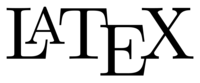
\includegraphics{latex.png}

\end{document}
